\chapter{Hexagonal Boron Nitride under strain}
\chaptertoc{}

\textit{This chapter is partly based on our publication Ref. \cite{lechifflart2022excitons}. Some of the text and figures contained in this Chapter are adapted from this reference.}

%
\section{Introduction and experimental motivations}
Strain is a powerful tool to engineer electronic and optical properties of materials. It is possible to modify the electronic dispersion of strained crystals, in particular to modify the conduction band minima and the valence band maxima, even leading to a direct to indirect bandgap transition, as it was shown for Germanium \cite{hoshina2009first,cheng2010strain} and more recently for transition metal dichalcogenides.\cite{desai2014strain,choudhary2020shear,frisenda2017biaxial} Regarding hBN, the effect of strain on vibrational properties was investigated experimentally in exfoliated hBN with various thicknesses,\cite{androulidakis2018strained} while theoretically biaxial tensile strain was considered for the mono- and bilayer h-BN \cite{yang2013distorted,fujimoto2016band} as well as its role on hexagonal boron nitride quantum emitters.\cite{tabesh2021strain} But little is known about the effect of strain on the optical properties of bulk h-BN, which are the simplest mean to characterize this material. \\
A recent experiment showed a remarkable modification of the cathodoluminescence spectrum of hBN under strain. \cite{schue2017proprietes} In this experiment Léonard Schué, from the group of Julien Barjon, suspended a nanosheet of hexagonal Boron Nitride over a trench carved out from an SiO$_2$ substrate. The nanosheet is about 100 nm thick and curves under the effect of gravity, as illustrated in Fig. \ref{fig:exp_strain}(a), and was imaged by \acrfull{AFM} (Fig. \ref{fig:exp_strain}(b)).
\begin{figure}[tbp]
	\vspace{0.2cm}
	\setcapindent{2em}
	\centering
	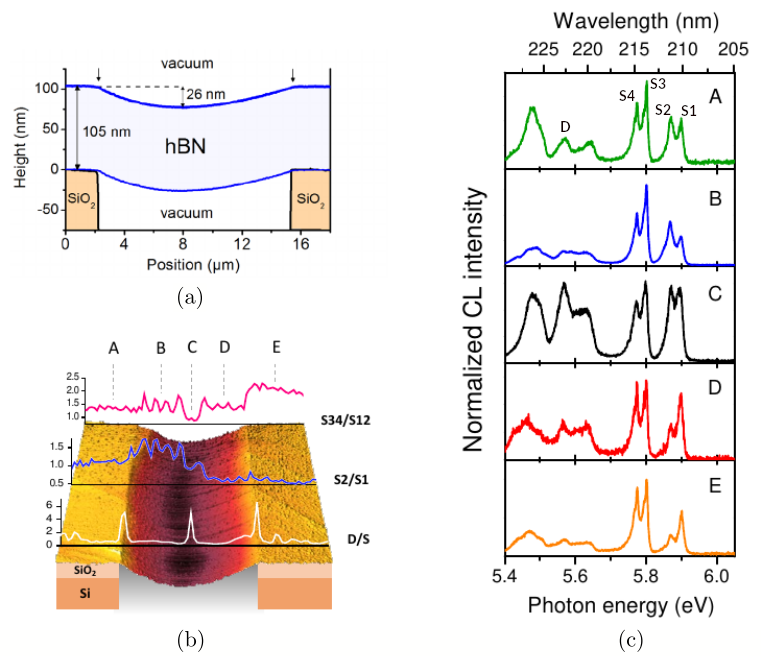
\includegraphics[width=0.7\textwidth]{exp_strain.png}
	\caption{(a) Sketch of the deposited hBN nanosheet on the trench. (b) AFM profile and relative intensity ratios of different emission peaks with respect to spatial region. (c) Cathodoluminescence intensity measured on different regions of the sample. Courtesy of Léonard Schué and Julien Barjon}
	\label{fig:exp_strain}
\end{figure}
When measuring the cathodoluminescence spectra at different positions on the sample, one can see that the intensity ratios between different peaks are varying. Their interpretation is that the deformation of the sample induces uniaxial (compressive) strain, perpendicular to the trench. This strain could have an effect on the recombination process of excitons or their scattering with phonons, leading to a change in the luminescence intensity. They measure an intensity ratio between the S1/2 and the S3/4 peaks varying from $\approx 4$ at equilibrium to almost 1 at the bottom of the trench. We try to simulate this phenomenon and use a finite difference method to reproduce the phonon-assisted luminescence in strained structures from first principles.

%
\section{Structure and phonons}
In order to simulate the hBN sample in suspension, we consider an infinite bulk crystal under uniaxial strain. In the experiment, the beam of electron penetrates only on the upper part of the nanosheet, where the strain is compressive. However for the first steps of the computational workflow, we study a range of strain including both stretching and compression around the equilibrium structure.
First, we obtain the strained structure by taking an orthorombic cell of the pristine crystal, larger than the hexagonal unit cell. Because it has three orthogonal lattice vectors, the orthorombic cell is more suited for the application of a uniaxial strain. To do so, we simply alter the length of one cell vector, up to an arbitrary length corresponding to a value of strain. We studied different strain values, in an interval going from a $+2.5\%$ to a $-2.5\%$ variation of the equilibrium length. In this work we applied strained in the armchair direction, the one parallel to the B-N bond. 
\begin{figure}[tbp]
	\vspace{0.5cm}
	\setcapindent{2em}
	\centering
	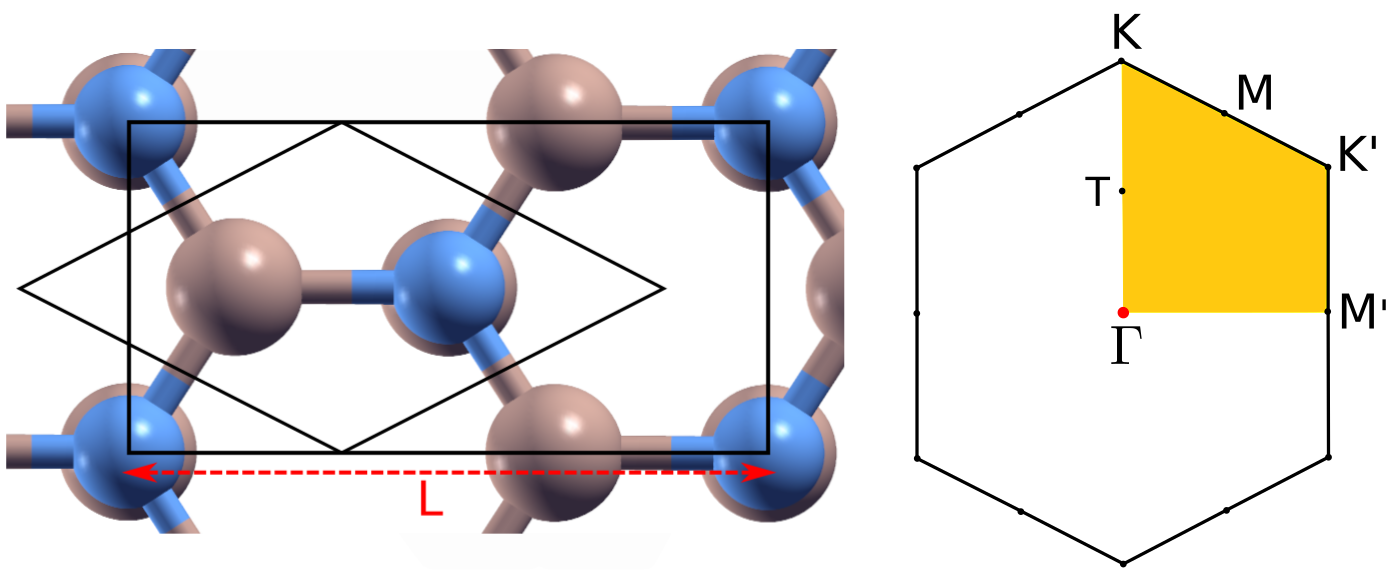
\includegraphics[width=0.8\textwidth]{AppB_structure_BZ.png}
	\caption{Left : visualization of the strained crystal and the orthorombic and pseudo-hexagonal unit cells. Right : corresponding strained Brillouin Zone. The dotted line is the shape of the equilibrium BZ. The yellow zone is the area enclosed by the high-symmetry points we used to plot dispersions. \textcolor{red}{maybe add phonon density of states (from suppmat) on the side}}
	\label{fig:strain_BZ}
\end{figure}
After setting the length of the cell to the desired length corresponding to a strain value, we let the atom positions and the other two cell vectors relax, using a damped molecular dynamics algorithm where the forces acting on the atoms are computed in \acrshort{DFT} using the Hellmann--Feynman theorem. This procedure in implemented in the \qe ~suite.\cite{giannozzi2009quantum,giannozzi2017advanced} More computational details can be found in Appendix \ref{app:comp_par_strain}. We found that once the two cell vectors orthogonal to the strained one are relaxed, their length vary linearly with the strain.\\
Once we have the relaxed strained orthorombic cells, we construct a pseudo-hexagonal unit cell containing only four atoms. This way, we can compare the structures obtained for different strain values with the equilibrium structure in a consistent way and proceed with the calculation of electronic and optical properties. To construct the pseudo-hexagonal cells from the strained orthorombic ones, we followed the procedure described in Appendix \ref{app:ortho2hex}. We computed the phonon-related properties using \acrshort{DFPT} in the four-atom strained cells. In the strained crystal, whatever the value of strain, the 120\textdegree~ rotational symmetry is broken and this makes the \MM~and \KK~points in the \acrshort{BZ} nonequivalent to the \MM' and \KK' points. The path between high-symmetry points containing all four of these points is drawn in yellow in Fig. \ref{fig:strain_BZ}.
The resulting phonon dispersions are shown in Fig. \ref{fig:strain_phonons}, for three strain values : a $+2.5\%$ stretch, a $-2.5\%$ compression and the equilibrium one.
\begin{figure}[tbp]
	\vspace{0.5cm}
	\setcapindent{2em}
	\centering
	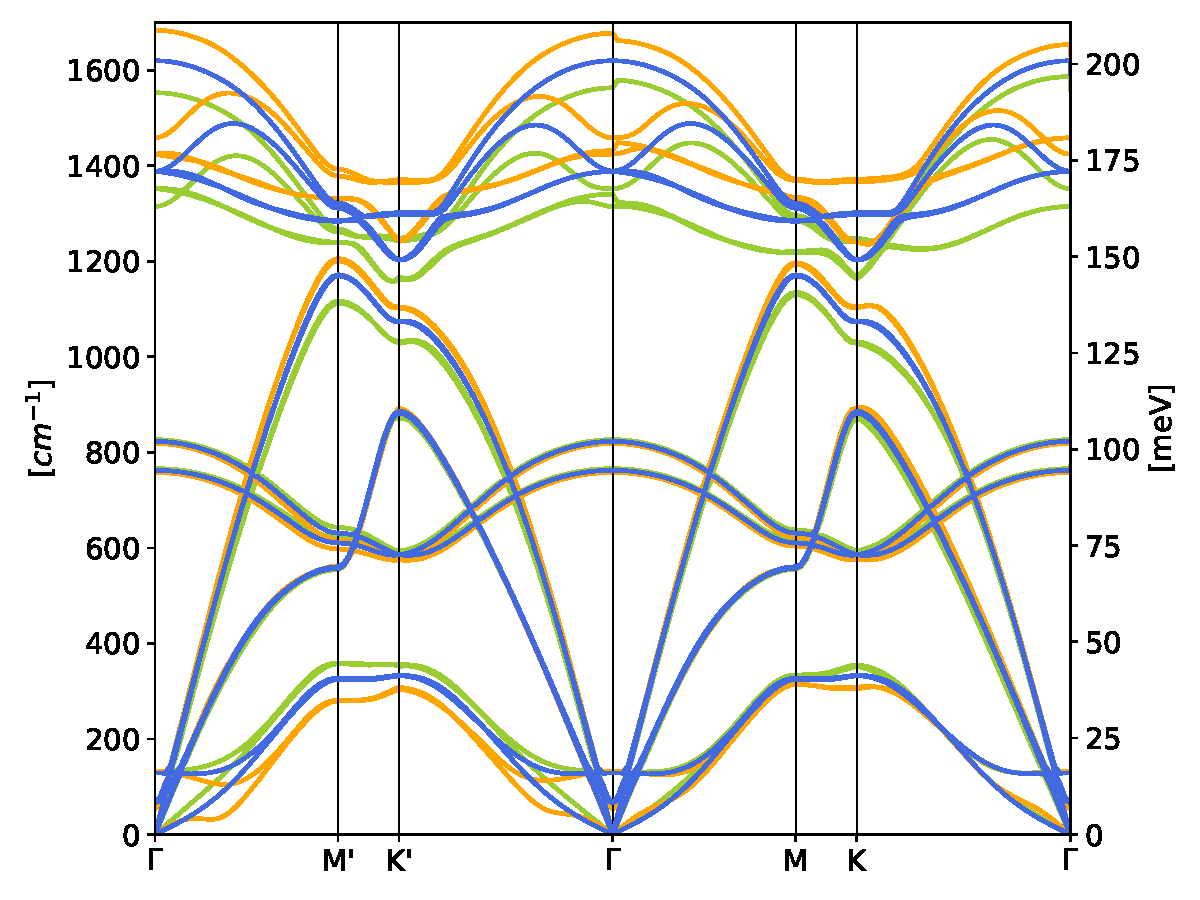
\includegraphics[width=0.8\textwidth]{strain_ph.pdf}
	\caption{Phonon dispersion versus uniaxial strain. Blue lines are at equilibrium, green lines at 2.5\% stretch and orange lines at 2.5\% compression.}
	\label{fig:strain_phonons}
\end{figure}
For the unstrained dispersion we can notice the splitting of the highest branch at $\Gamma$ with the two branches below. This is the LO-TO splitting mentioned in Sec. \ref{sec:DFPT}.

We found that the optical modes (the branches with the highest energies) are the most affected by strain. With compressive strain, their frequencies are increased at all $\qq$ points and they are decreased for tensile strain. We also observe the splitting of the E$_{2g}$ modes, whose frequencies are degenerate at $\Gamma$ just below 175 meV (1400 cm$^{-1}$) for the unstrained structure. They split as soon as a strain is applied. This is in agreement with Raman measurements and previous calculations.\cite{blundo2022vibrational,androulidakis2018strained} It is also interesting to notice that depending on the direction along which the $\Gamma$ point is approached, the splitting of the two E$_{2g}$ modes has different magnitudes. 

On the mid-energy range of the dispersion, the LA, TA and TO modes are not very affected by strain. This will be important in the discussion about luminescence in the following.

On the lower frequency end, the acoustic modes are affected in an opposite way. Under compression, their frequencies are decreased and increased under stretch. The orange curve shows a softening of the lowest branch close to $\Gamma$. We noticed that increasing the value of compressive strain leads to the appearance of negative frequencies. This happens when the geometry is unstable. Then the second derivative in Eq. \eqref{eq:IFC_matrix} is negative and the eigenvalues $\omega^2$ in Eq. \eqref{eq:ph_evprob} are negative. The imaginary solutions would be plotted as negative, by convention. We did not investigate this instability caused by compression, since the range of strain we are interested in is below $+2.5\%$ of strain. Nonetheless, the phonon dispersions show that our systems are stable in the range of strain considered.

%
\section{Electronic structure}
In order to study the electronic structure of strained hBN, we first compute the Kohn-Sham eigenvalues in \acrshort{DFT} and then we performed a one-shot G$_0$W$_0$ calculation to compute the quasiparticle corrections using the \yambo code.\cite{Sangalli_2019} We found that these corrections are a rigid shift in energy of the KS eigenvalues, independent of the strain applied in the range we considered. 
\begin{figure}[tbp]
	\vspace{0.5cm}
	\setcapindent{2em}
	\centering
	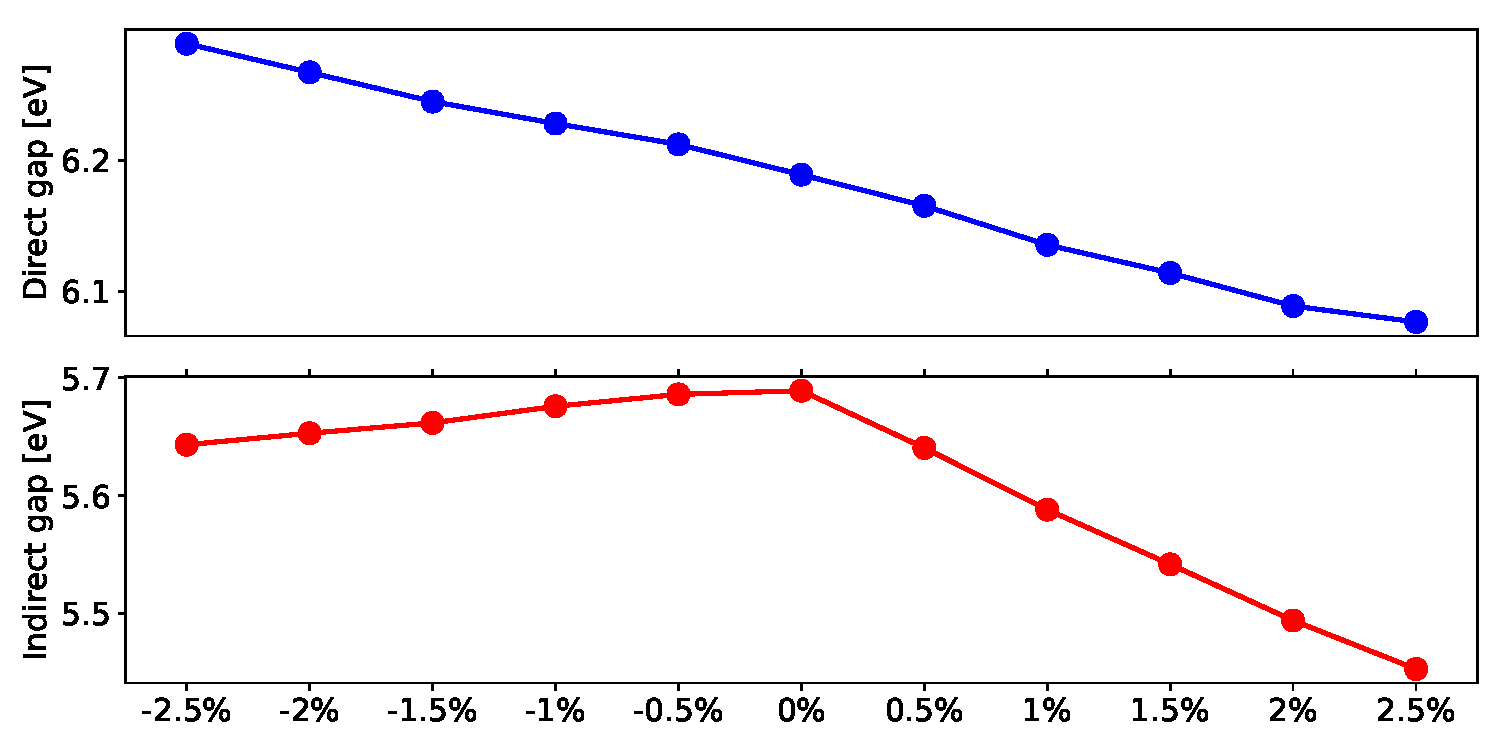
\includegraphics[width=0.8\textwidth]{strain_gw_gaps.pdf}
	\caption{Quasiparticle corrections to the direct and indirect bandgaps at the G$_0$W$_0$ level with respect to strain.}
	\label{fig:strain_gw_gaps}
\end{figure}
In Fig. \ref{fig:strain_gw_gaps} we report the variation of the direct gap (at \MM) and of the indirect gap (between \KK~and \MM) with respect to strain. The direct gap decreases linearly with increasing relative values of strain, while the indirect gap is maximal for the unstrained system and decreases both for compression and stretch.

The electronic dispersions along the path shown in Fig. \ref{fig:strain_BZ} are plotted in Fig. \ref{fig:strain_eldisp} for the two maximally strained systems and for the unstrained one. 
\begin{figure}[tbp]
	\vspace{0.5cm}
	\setcapindent{2em}
	\centering
	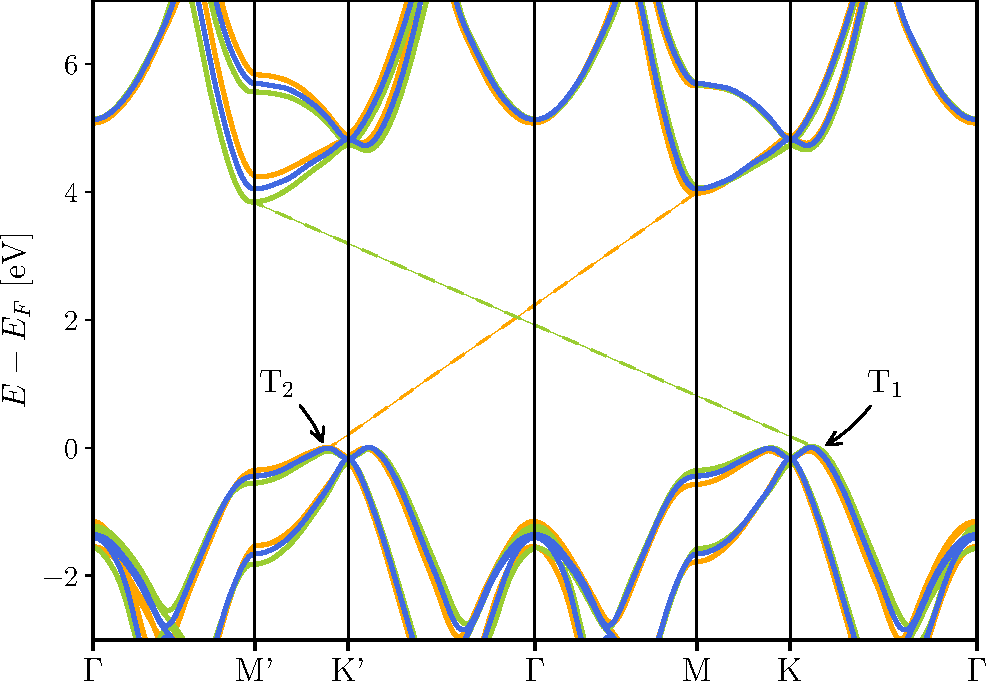
\includegraphics[width=0.6\textwidth]{strain_bands_qgaps.pdf}
	\caption{Details of the electronic band structure under the maximum
	stretch and compression considered in the manuscript. Blue lines are at equilibrium, green lines at +2.5\% stretch and orange lines at -2.5\% compression. We report also the location of the new indirect gaps in the two cases. Notice that at equilibrium all indirect transitions between the different \KK~ and \MM~ points are equivalent.}
	\label{fig:strain_eldisp}
\end{figure}
At equilibrium, the direct gap is located between states with a momentum close to \KK. The indirect gap is between a point close to \KK~for the valence band and the \MM~point for the conduction band. As discussed above, strain breaks one of the symmetries of the crystal and this effect is visible on the dispersions at high-symmetry points. Under compression, the conduction band is shifted down at \MM~while it is increased at \MM'. This trend is reversed under stretch. Hence, the conduction band minimum is at \MM~for the compressed crystal and at \MM' for the stretched crystal. 
These variations can be explained in term of the variation of the orbital properties. 
\begin{wrapfigure}{r}{0.41\textwidth}
	\vspace{-16pt}
	\setcapindent{1em}
	\centering
	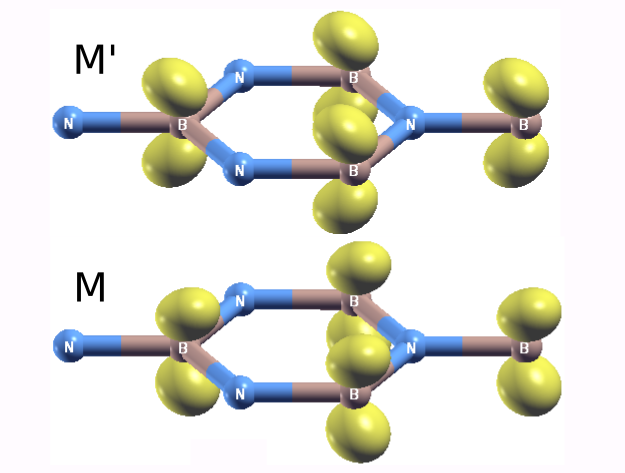
\includegraphics[width=0.4\textwidth]{M_and_M_prime.png}
	\caption{$\pi^*$ atomic-like orbitals of the conduction band minima on one of the layers for a compression of 0.5\%. At \MM', the components of the wavefunctions are oriented along the compressed B-N bond. At \MM, they are oriented along one of the other bonds.}%\textcolor{red}{Rajoute des flèches pour montrer le strain.}}
	\label{fig:WF_strain}
\end{wrapfigure}
The $\pi^*$ atomic-like orbitals at \MM~and \MM' have a different shape, as illustrated in Fig. \ref{fig:WF_strain} for a compression of 0.5\%. While they are degenerated in energy for the unstrained crystal, this degeneracy is lifted due to the symmetry breaking. The state with orbital components along the strained bond is the one whose energy changes with strain at \MM'. Moreover these orbitals have a strong dependence on the interlayer interactions,\cite{kang2016unified} which in turns depends on the interlayer distance. This distance varies linearly with the strain applied to the system in our relaxation process. These two effects, the breaking of the in plane symmetries and the change in the interlayer interaction, explain the splitting and shift of the bands induced by strain at the \MM' point.

The valence states around \KK~and \KK' are only slightly changed in energy. This can be explained because the orbitals corresponding to these states are protected from interlayer interactions by symmetry, as shown in the theoretical study of Ref. \cite{kang2016unified}. There is nonetheless a slight change in energy, which causes the valence band maximum to be located at the point called \textbf{T}$_2$ under compression and at \textbf{T}$_1$ under stretch. %\textcolor{red}{change the names either of these points OR of the T point in the BZ scheme}. 
All these modifications of the band structure induce a change in the position of the minimal indirect band gaps for compressive and tensile strain that are indicated by the dotted lines in Fig. \ref{fig:strain_eldisp}.


%
\section{Excitons and absorption}
On the low-energy end of the excitonic spectrum (in the sense of linear algebra) of bulk \acrshort{hBN}, we find two pairs of degenerate excitons. The splitting between the pairs is caused by the interlayer interactions and is called the Davydov splitting.\cite{paleari2018excitons} The two pairs transform differently under inversion operation (\textit{i.e.} taking $\rr \to -\rr$ or $\kk \to -\kk$), as explained in Appendix \ref{app:exc}. The lowest pair is even for inversion symmetry, which means it is dark in absorption. The second lowest pair instead is odd for inversion symmetry and thus bright.
Note that this is true for one-photon absorption, at the linear response level. In non-linear optics, for instance two-photon absorption, the dark and bright characters are reversed.\cite{attaccalite2018two} \\
The 120\textdegree~rotation symmetry breaking induced by uniaxial strain has an effect on the degeneracy of the Davydov pairs. First, looking at the energies of the four lowest excitons at $\Gamma$, as displayed in panel $(a)$ of Fig. \ref{fig:exc_abs_vs_strain}, we see that the energies are split, both for compression and stretching. 
These changes in energy are mainly due to the change in electronic gap reported in the above section. Indeed, they follow the same linear trend as the strain value increases and are of the same magnitude, about $\pm 0.1$ eV. We could also verify that the binding energies of the direct excitons remain approximately constant on the strain range considered, varying only by 10 to 15 meV.
\begin{figure}[tbp]
	\vspace{0.2cm}
	\setcapindent{2em}
	\centering
	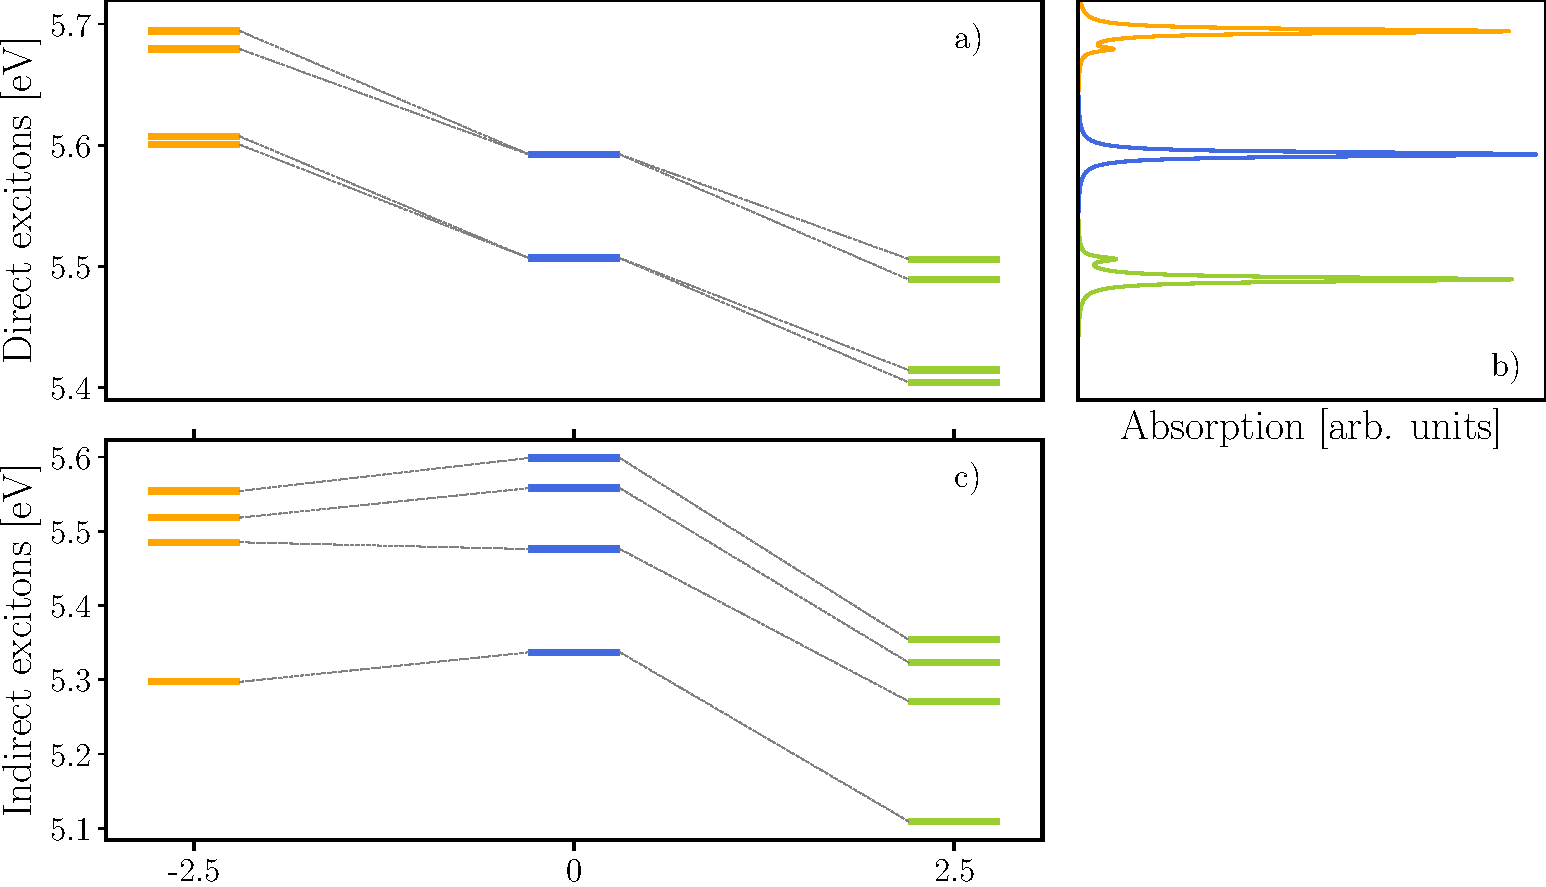
\includegraphics[width=0.8\textwidth]{hBN_exc_abs_vs_strain.pdf}
	\caption{Blue lines are for equilibrium crystal, orange is for compression and green is for stretch. (a) Energies of the lowest 4 excitons at $\Gamma$ (b) Absorption spectra associated with the direct excitons. Both excitons of the bright Davydov pair have a non-zero dipole matrix element and we can distinguish two peaks in the spectra for the strained crystals. (c) Energies of the lowest 4 indirect excitons.}
	\label{fig:exc_abs_vs_strain}
\end{figure}

The associated absorption spectra are displayed in panel (b) of Fig. \ref{fig:exc_abs_vs_strain}. As the inversion symmetry is not broken by uniaxial strain, the lowest two excitons remain dark when strain is applied. For the third and fourth lowest excitons in the strained systems, they are not degenerate anymore, as it is the case in the pristine crystal, due to the breaking of rotational symmetry. This gives both excitons a non-zero dipole, and we see two peaks appearing in the absorption spectra. \\
The change of peak energy induced by strain is quantified by the strain gauge factor, which is defined as the spectral shift per \% of uniaxial strain. From our calculations, we find a value of $\approx$ 43 meV/\%, which is in the same range as transition metal dichalcogenides as reported in Ref. \cite{carrascoso2021strain}.

The splitting is also visible on the exciton wavefunctions in real space. It is displayed in Fig. \ref{fig:excWF_strain} for the lowest two excitons at $\Gamma$, for a stretch of +2.5\%. In the pristine crystal, these two wavefunctions are mixed. Here the splitting is clear, with one of the wavefunctions having its components along the strained B-N bond or the armchair direction, while the other has its components along the zigzag direction.
\begin{figure}[tbp]
	\vspace{0.2cm}
	\setcapindent{2em}
	\centering
	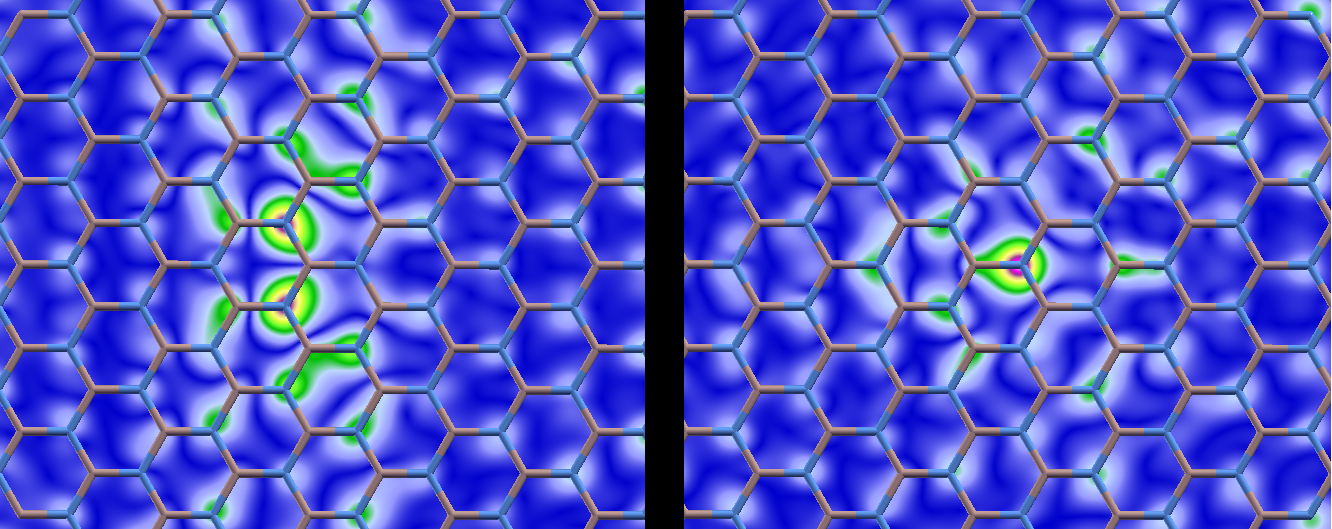
\includegraphics[width=0.8\textwidth]{excitonWF_strain.png}
	\caption{Electron distribution when the hole is fixed near the central Nitrogen atom, that we call exciton wavefunction. Left is the lowest dark exciton at $\Gamma$, right is the second lowest dark exciton at $\Gamma$, taken for a stretch of +2.5\%. Note that the wavefunctions of the lowest bright excitons, not shown here, have the same structure as the dark ones}
	\label{fig:excWF_strain}
\end{figure}

We observe the same trend for the lowest-lying excitons with non-zero momentum, which we will call indirect excitons because they are formed by indirect electronic transitions. Their change in energy with strain is reported in Fig. \ref{fig:exc_abs_vs_strain} (c). It follows the same variation as the indirect gap and here again their binding energy is almost invariant with strain. The indirect excitons of hBN play an important role in light emission by luminescence. These changes in energy combined with the change in phonon frequencies will have an impact on the luminescence spectra of the strained crystals. This will be discussed in the next two sections.

%
\section{Exciton-phonon coupling from finite differences} \label{sec:excph_fdd}
As presented in the introduction of the thesis, the inclusion of lattice vibrations in our computational framework is necessary to describe accurately the phonon-assisted features in the luminescence spectrum of hBN. In particular the exciton-phonon coupling is the central quantity to take into account. To do so, I present in this section how to calculate the macroscopic dielectric function with a static correction due to lattice vibrations, in a finite-difference scheme. The method can be found in Ref. \cite{paleari2019exciton} and in a slightly different approach in Ref. \cite{cannuccia2019theory}.\\
The key idea is to take the Taylor expansion of the macroscopic dielectric function with respect to atomic displacements. By displacing the atoms around their equilibrium positions along the phonon eigenvectors obtained earlier with \acrshort{DFPT} and calculating the response function with the \acrshort{BSE} in the displaced configurations, we will obtain the coupling between the exciton responsible for the optical response and the phonons. The link between the response function and the macroscopic dielectric function is given by Eq. \eqref{eq:eps_macro}. \\
Our goal is to write the dielectric constant as a term at equilibrium
plus a correction due to the atomic motion as $\varepsilon (\omega)\approx \varepsilon^{(0)}(\omega) + \varepsilon^{st,(2)}_{\bar{q}}(\omega)$, where the second term is the static correction induced by the atomic displacements, and it will be averaged over the displacements along all phonon modes.\cite{zacharias2016one} 
The contribution from exciton $\lambda$ to the response function  writes :
\begin{equation}
	\chi^\lambda_{R=0}(\omega) = \frac{|T^\lambda_{R=0}|^2}{E^\lambda_{R=0} - \omega + i \eta} \label{eq:chi_R_lambda}
\end{equation}
where the subscript $R=0$ indicates that the quantities are evaluated at clamped ion positions. The infinitesimal $\eta$ is taken independent of $R$ for simplicity.
The single-exciton contribution can be highlighted by writing :
\begin{align}
	\chi_{R=0}(\omega)&= \sum_\lambda \chi^\lambda_{R=0} (\omega),  \label{eq:chi} \\
\epsilon_M(\omega)&=1 -  \hat d \chi_{R=0}(\omega) \hat d = 1 - 4\pi\sum_\lambda \frac{ | T_{R=0}^\lambda|^2}{\omega - E^\lambda_{R=0} + i\eta},
\end{align}
where $\hat{d}$ is the dipole operator with matrix elements $d_{cv\kk} = \langle v \kk | \hat r | c\kk \rangle$ and the exciton dipoles are defined as $T^\lambda = \sum_{cvk} \bar{A}_\lambda^{cvk} d_{cvk}$. The first derivative entering in the Taylor expansion will be :
\begin{equation}
	\frac{\partial \chi^\lambda_R(\omega)}{\partial R}\biggr|_{R=0} = \frac{\partial |T^\lambda_R|}{\partial R}\biggr|_{R=0} \frac{2|T^\lambda_{R=0}|}{E^\lambda_{R=0} - \omega + i\eta} + \frac{\partial \left[ E^\lambda_R - \omega + i\eta \right]^{-1}}{\partial R}\biggr|_{R=0} |T^\lambda_{R=0}|^2.
\end{equation}
This expression has a term linear in the exciton dipole and a term at the second power, both taken at clamped ion positions. It means that for dark excitons, the first derivative in the Taylor expansion will be zero, but it can have a non-zero contribution for bright excitons, for a discussion see Refs. \cite{zacharias2016one,zacharias2015stochastic}. Dark excitons are labelled $\lambda'$, and we have $\frac{\partial \chi^{\lambda'}_R(\omega)}{\partial R}\bigr|_{R=0} = 0$.
In \acrshort{hBN}, the excitons involved in luminescence are the ones with the lowest energies in the finite momentum dispersion. Because of momentum conservation, they cannot recombine and emit light which has almost zero momentum, hence they are dark at clamped ion positions. Phonons are needed to transfer momentum and assist their recombination. \\ 
Similar arguments hold for the second derivative in the Taylor expansion
and the only non-vanishing term that remains is :
\begin{equation}
	\frac{\partial^2 \chi^{\lambda'}_R(\omega)}{\partial R^2} = \frac{\partial^2 |T^{\lambda'}_R|^2}{\partial R^2}\biggr|_{R=0} \left[ E^{\lambda'}_{R=0} - \omega + i\eta \right]^{-1} \label{eq:chi_fdd}
\end{equation}
This equation shows that it is equivalent to compute the finite-difference derivative of the full response function or only of the exciton dipoles if we are only interested in corrections up to the second order. This was verified numerically in Ref. \cite{paleari2019exciton}. In our calculations, we compute the derivative of the dipoles since they can be obtained more easily in the code. \\
This above second derivative is evaluated numerically with the finite difference formula :
\begin{equation}
	\frac{\partial^2 \chi^{\lambda'}_R(\omega)}{\partial R^2} \approx \frac{\chi(\Delta\RR;\omega) - 2 \chi_0(\omega) + \chi(-\Delta\RR;\omega)}{\Delta\RR^2}
\end{equation}

Since we are interested in phonon-assisted luminescence and we know where the minima lie in the excitonic dispersion, we know the phonon momentum $\bar{q}$ necessary to satisfy momentum conservation. Therefore we calculate the derivatives of the excitonic dipoles
only for a momentum $\bar{q}$ that connect the minimum of the exciton dispersion to $\Gamma$ as illustrated in Fig. \textcolor{red}{exc disp and phonon arrow at $\bar{q}$}.
Then we label the displacements $R \to R_{\mu\bar{q}}$. They are along the eigenvector of a particular phonon mode $\mu$ taken at the momentum $\bar{q}$. The displacement magnitudes are given, similarly to Eq. \eqref{eq:normal_displacements} taken for $t=0$, by the real part of the phonon eigenvector multiplied by a scaling factor $c$ :
\begin{equation}
	u^{\mu\bar{q}}_{Ls\alpha}(t=0) = \frac{c}{\sqrt{M_s}}\Re\left\{ e^{i\bar{\qq}\cdot\boldsymbol{\tau}_L} \xi^{\mu\bar{q}}_{s\alpha} \right\}
\end{equation}
The $c$ parameter is a scaling factor which needs to be converged. Indeed for the finite difference derivative, we want to keep the displacements as small as possible. However if they are too small, their effect will be indistinguishable from numerical noise, but if they are too large, effects beyond the second-order derivatives will start to appear. For this work, we converged the displacements to a value of $|\Delta \RR| = 0.05$ \AA.
To accommodate the periodicity of the phonon at $\bar{q}$, we construct supercells that map the $\bar{q}$ point at $\Gamma$. These supercells are non-diagonal in general,\cite{lloyd2015lattice} and we build them using the \texttt{yambopy} Python tool.\cite{Sangalli_2019} Note that we approximate the momentum $\bar{q}$ so that its vector coordinates are accommodable in reasonably small supercells.\\
From Ref. \cite{zacharias2020theory}, the second-order correction to the full dielectric due to the transitions assisted by a single phonon of momentum $\bar{q}$ is :
\begin{equation}
	\varepsilon^{st,(2)}_{\bar{q}} (\omega) = \frac{1}{2} \sum_\mu \left[ \sum_i^{N_{\bar{q}}} \frac{1}{2} \sum_j^2 \frac{\partial^2 \varepsilon^{(0)}_j(\omega)}{\partial R^2_{\mu\bar{q}}} \biggr|_{eq} \right] \sigma^2_{\mu\bar{q}} \label{eq:eps_Taylor_2nd}
\end{equation}
where $j$ is the polarization direction of the incoming light. We average over two orthogonal in-plane directions. The index $i$ runs over the equivalent $\bar{q}$ points in the \acrshort{BZ} where the exciton energies are minimal. For a perfect hBN crystal, $N_{\bar{q}} = 6$ but in our case, $N_{\bar{q}} = 4$. The last factor $\sigma^2_{\mu\bar{q}}$ is the thermal average of the squared displacement of the a quantum harmonic oscillator, given by :
\begin{equation}
	\sigma^2_{\mu\bar{q}}(T) = l^2_{\mu\bar{q}} (2n_{\mu\bar{q}}(T) + 1).
\end{equation}
$n_{\mu\bar{q}}(T)$ is the Bose-Einstein occupation function, and $l^2_{\mu\bar{q}} = 1/(2M_{\mu\bar{q}}\Omega_{\mu\bar{q}})$ is the zero-temperature squared displacement (from now on we refer to phonon frequencies with capital Omega). In our case the reference mass is $M_{\mu\bar{q}} = \sum^{N_{ions}}_s M_s |\xi_s^{\mu\bar{q}}|^2$.\\
Finally the imaginary part of the dielectric function follows from Eqs. \eqref{eq:chi_fdd},\eqref{eq:chi_R_lambda} and \eqref{eq:eps_macro} : 
\begin{equation}
	\Im\frac{\partial^2 \varepsilon^{(0)}(\omega)}{\partial R^2_{\mu\bar{q}}}\biggr|_{eq} = \frac{8\pi}{N_k V} \sum_{\lambda'} \frac{\partial^2 |T^{\lambda'}|^2}{\partial R^2_{\mu\bar{q}}}\biggr|_{eq} \Im\left\{ \frac{1}{\omega - E^{\lambda'} + i\eta} \right\}.
\end{equation}
At this point we can reintroduce the dependence on the phonon frequency coming from the energy conservation in perturbation theory, which was neglected above (more details can be found in Ref. \cite{paleari2019first}). Two terms appear, one coming from the process of phonon emission which is proportional to $1 + n_{\mu\bar{q}}$ and one from phonon absorption proportional to $n_{\mu\bar{q}}$. We have the transformation :
\begin{equation}
	\frac{2n_{\mu\bar{q}} + 1}{\omega - E^{\lambda'} + i\eta} \to \frac{n_{\mu\bar{q}} + 1}{\omega - E^{\lambda'} - \Omega_{\mu\bar{q}} + i\eta} + \frac{n_{\mu\bar{q}}}{\omega - E^{\lambda'} + \Omega_{\mu\bar{q}} + i\eta}
\end{equation}
At low temperature, $1 \gg n_{\mu\bar{q}}$ which means that absorbing a phonon is much less likely than emitting one. 
The final expression writes :
\begin{equation}
	\varepsilon^{(2)}_{\bar{q}2}(\omega) = \frac{8\pi}{N_k V} \sum_{\lambda'} \frac{\partial^2 |T^{\lambda'}|^2}{\partial R^2_{\mu\bar{q}}}\biggr|_{eq} l^2_{\mu\bar{q}} \left[ n_{\mu\bar{q}} + 1/2 \mp 1/2 \right] \delta(\omega - E^{\lambda'} \pm \Omega_{\mu\bar{q}}). \label{eq:eps2_fdd}
\end{equation}
The upper (lower) sign refers to the process of phonon absorption (emission). One thing to note here is that we neglect the variation of the exciton energies induced by the coupling with phonon, which is an effect beyond second order derivative for indirect excitons, so we expect this renormalization to be minor.\cite{marini2008ab} Moreover we know that due to the approximations adopted in this work we will not be able to get the correct absolute position\cite{artus2021ellipsometry} of the exciton but only the relative position of indirect emission with respect to the direct one. 

%
\section{Luminescence results}
In order to compute the luminescence spectra, we used the van Roosbroeck--Shockley relation from Eq. \eqref{eq:vRS_PL_ind} combined with the expression of the dielectric function in Eq. \eqref{eq:eps2_fdd}. We simulate a crystal at low temperature, which we set at 10K in agreement with the experimental measurements. At this temperature, the phonon emission processes widely dominate the absorption ones and we have $n_{\mu \bar{q}} \ll  1$. Therefore we set these factors to zero in the numerator. We get a final expression for the luminescence as :
\begin{multline}
	R^{sp}(\omega)= \mathcal{D} \sum_{\mu,{\bar{q}}} \frac{\omega(\omega + 2\Omega_{\mu \bar{q}})^2}{\pi c^3 } n_1(\omega) \sum_{\lambda'} \frac{\partial^2 |T^{\lambda'}|^2 }{\partial R_{\mu\bar{q}}^2}\biggr|_{\text{eq}} \\ \times	\Im \left\{\frac{1}{\omega-(E^{\lambda'}-\Omega_{\mu \bar{q}})+i\eta}\right\} n_B(E^{\lambda'}_{\bar{q}},T_{exc}) \label{eq:strain_vRS_PL}
\end{multline}
where $\mathcal{D}$ is a dimensional factor, $n_B(E^{\lambda'}_{\bar{q}},T_{exc}) = e^{-(E^{\lambda'}-E^{min})/k_BT_{exc}}$ is the Boltzmann occupation for excitons where the energy difference is taken with the minimal exciton energy over the whole Brillouin Zone $E^{min}$. Except for a multiplicative factor, the formula for the luminescence is equivalent to the phonon-assisted absorption one, with the difference that excitons are weighted by an occupation factor. It means that the lowest valleys in the exciton dispersion will be populated by relaxed excitons, while the higher states will have exponentially decaying populations.
For instance, the direct exciton has an energy too large to even be visible in the spectrum.
\\
The excitonic temperature $T_{exc}$ is higher than the lattice temperature because we consider a steady-state process in which the excitons do not thermalize, since they are constantly pumped by the laser. We obtained the value by fitting the experimental data of Ref. \cite{cassabois2016hexagonal} which gave us the value of $T_{exc} = 24 K$ for a lattice temperature of $T_L = 10 K$. The effect of temperature is also taken into account in the broadening parameter of the peaks with the Lorentzian model : $\eta = \Gamma_0 + aT + bB(T)$ where the values of the parameters can be found in Refs. \cite{paleari2019exciton,vuong2017exciton}. Another approximation we made is to compute the dipoles at the displaced configurations with the statically screened interaction from the equilibrium configurations : 
\begin{equation}
	\frac{\partial^2 |T^{\lambda'} (W, L )|^2 }{\partial R_{\mu \bar{q}}^2} \simeq \frac{\partial^2 |T^{\lambda'} (W(R=R_{eq}), L) |^2 }{\partial R_{\mu \bar{q}}^2}.
\end{equation}
It has been shown previously that this has negligible effects for the calculation of electron-phonon matrix elements,\cite{faber2015exploring} and we verified that our results are not modified by this approximation. 

Now comes the discussion about the choice of $\bar{q}$. For the pristine hBN crystal, the indirect electronic gap is between two points close to the \KK~point and the \MM~point. The usual approximation is to consider that the gap lies on the \KK~point, and that the momentum that connects the two points is $\qq = (\tfrac{1}{3}, -\tfrac{1}{6}, 0)$ and that the minimum of the exciton dispersion is also at this momentum. It has been shown to be a reliable approximation.\cite{cannuccia2019theory,paleari2019exciton} This simplifies the construction of the supercells needed to accommodate the phonon modes at this $\qq$-vector. In our case, because of the symmetry breaking in the electronic dispersion, there are several indirect gaps which have a very similar energy, especially for low values of strain. This could lead to a broadening of the peaks in the luminescence spectra. In order to verify this hypothesis, we constructed the supercells which accommodate all the vectors corresponding to the transitions $\bf M - \bf K$,  $\bf M - \bf {K'}$,  $\bf {M'} - \bf K$ , $\bf {M'}  - \bf { K'}$. Then we performed a \acrshort{BSE} calculation for all these non-diagonal supercells containing 24 displaced atoms and summed the dipoles. Because of the displacement of atoms, some symmetries are broken and the dark excitons which are folded at $\Gamma$ acquire a finite dipole, hence contributing to the luminescence spectra.\\

The resulting spectra for various values of strained are displayed in Fig. \ref{fig:Lum_vs_strain}.
\begin{figure}[tbp]
	\vspace{0.2cm}
	\setcapindent{2em}
	\centering
	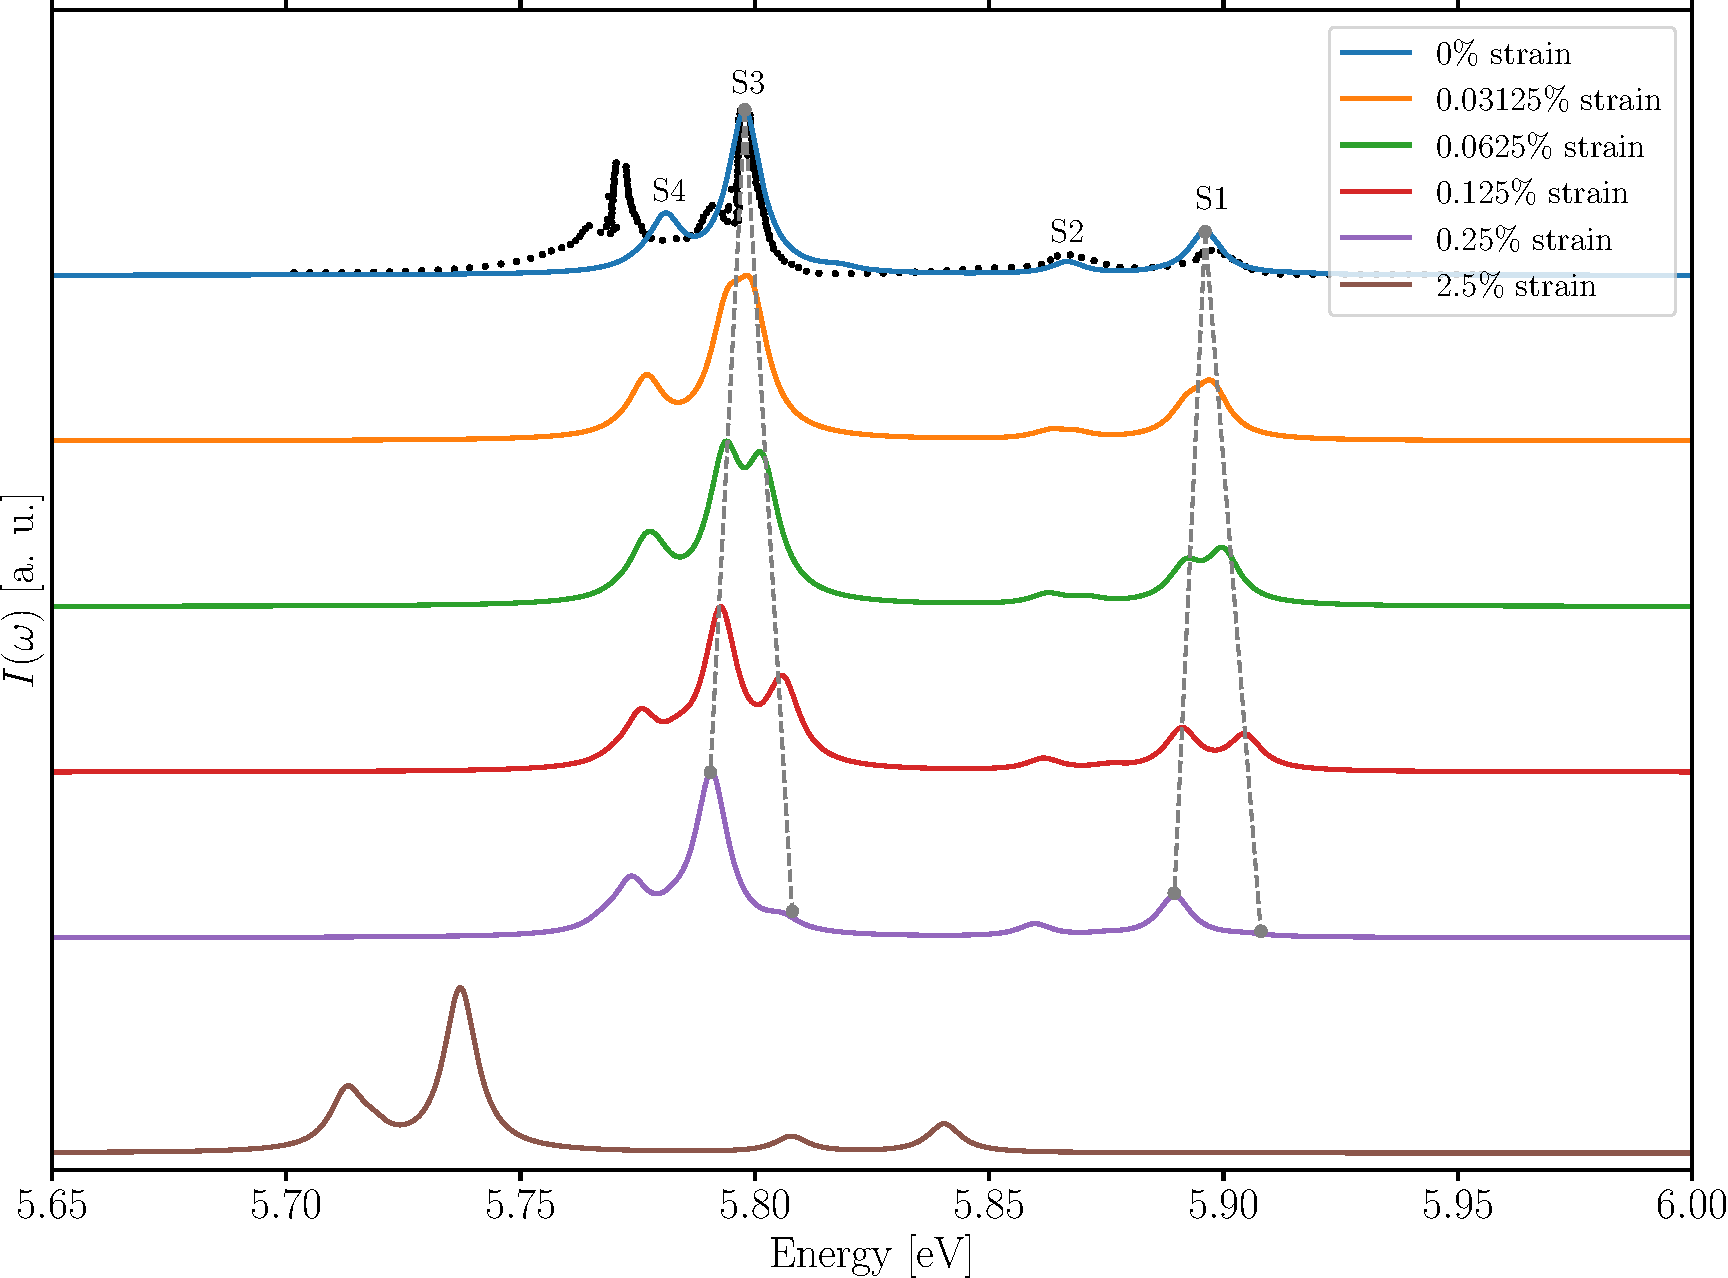
\includegraphics[width=0.9\textwidth]{Lum_vs_strain.pdf}
	\caption{Luminescence spectra as a function of strain, for selected value of compressive strain. Plots are shifted vertically for clarity. On the top plot, experimental data is represented by the black dots from Ref. \cite{schue2019bright}. The spectra have been shifted to match the position of the indirect exciton at equilibrium, and compensate the numerical error of the $GW$ approximation.\cite{artus2021ellipsometry} Dashed lines are a guide for the eye.}
	\label{fig:Lum_vs_strain}
\end{figure}
First, we can see on the top plot that the equilibrium luminescence spectrum is quite well reproduced compared to experiment. At low values of strain, the excitons originating from the different $\bf{ M^{(')}} - \bf{ K^{(')}}$ transitions have a very close energy and therefore all of them contribute to the luminescence spectra as they are not suppressed by the Boltzmann function. These excitons scatter with phonons who also have their frequencies modified. These combined effects create a splitting of the peaks which increases with strain. There is also a slight increase in the intensity of the S1 and S2 peaks, coming from scattering with LA and TA modes. At equilibrium, we found that the S3/S1 intensity ratio is $\approx 3.7$ and it decreases down to $\approx 2.7$ with strain. This result is in line with those of Léonard Schué in Ref. \cite{schue2017proprietes}, however they found a ratio going down to $\approx 1$ in their compressed samples.\\ 
The discrepancy could be explained by the lack of the fine sampling of the exciton and phonon dispersions. Indeed with a larger density of states to scatter, the intensity of some peaks could be increased even more. The differences could also come from experimental factors not accounted for in our simulation methods, such as surface effects or the fact that the strain field could be non-uniform and with an unknown direction, which we cannot reproduce with the uniaxial and homogeneous strain that we simulated.  

Finally, for larger values of strain, the exciton energies split so much that the peaks coming from the higher one are suppressed by the Boltzmann function in the van Roosbroeck--Shockley relation. The spectrum thus acquires the same shape as the equilibrium one but translated to lower energies due to the closure of the indirect gap, and the change in the phonon frequencies. Note that the $2.5\%$ value of strain is extreme and is probably out of reach in the experimental conditions we try to reproduce. The results are similar for the tensile strain.

%
\section*{Conclusion of the chapter}
In this chapter, I presented our results about the electronic, phononic and optical properties of bulk hBN under uniaxial strain, both tensile and compressive., along the armchair direction. We observed a splitting of the exciton at $\Gamma$ due to the breaking
of the threefold rotational symmetry. This splitting could be measured in reflectivity experiments.\cite{elias2021flat} We also found that the direct excitons energies vary linearly with the applied strain, while the indirect exciton energies decrease both with compression and stretch. We were also able to evaluate the strain gauge factor, which was found to be similar to that of transition metal dichalcogenides.
I presented a method to include the exciton-phonon coupling in the response function and hence in the optical spectra of the strained crystals. It is based on a finite-difference derivative approach and is well-suited for materials with a indirect and deep exciton dispersion exciton minimum. The coupling of excitons and phonons is calculated only for a few momenta in the Brillouin Zone. Since this method requires the use of supercells, it is particularly adapted to the study of defects such as in Ref. \cite{libbi2022phonon}. We employed the method to compute the phonon-assisted luminescence spectrum and how it changes with strain. We found that at low strain,additional peaks appear in the spectra due to the breaking of the degeneracy between the different \KK~ and \MM~ points in the Brillouin Zone. These additional peaks decrease the intensity ratio between the acoustic- and the optical-phonon assisted transitions, in agreement with recent measurements. For large compressive strain we found that only one valley contributes to the luminescence, and the spectra return to a shape similar to the equilibrium one but shifted at lower energies. This prediction could be verified by means of luminescence measurements in highly strained h-BN.\cite{blundo2022vibrational}